\documentclass[
xcolor={svgnames},
hyperref={colorlinks,citecolor=DeepPink4,linkcolor=Black,urlcolor=DarkBlue}
]{beamer}
\usepackage[utf8]{inputenc}
\usepackage[spanish]{babel} 
\usepackage{hyperref}
\usepackage{graphicx}

\usepackage{setspace}
\usepackage{xcolor}
%\usepackage{listings}
%\usepackage{minted}



\write18{mkdir images}


\usetheme{CambridgeUS}
\usecolortheme{seahorse} % https://www.hartwork.org/beamer-theme-matrix/
% \useoutertheme{shadow}
\useinnertheme{rectangles}

\AtBeginSection[]
{
	\begin{frame}<beamer>
		\frametitle{Índice}
		\tableofcontents[
			currentsection
		]
	\end{frame}
}


\title{Continuous Integration EGC}
\subtitle{AgoraUS - Grupo 1}
\author{
		Manuel Francisco López Ruiz
		  }
\institute[EGC]{
	Evolución y Gestión de la Configuración [EGC] \\
	Grado en Ingeniería Informática - Ingeniería del Software
	\and
	Universidad de Sevilla (Spain)
}

\begin{document}

\begin{frame}[plain]
	% Run with pdflatex --shell-escape 
	\titlepage
\end{frame}



\begin{frame}
	\frametitle{Índice}
	\tableofcontents
\end{frame}


\section{Introducción}

\begin{frame}
	\frametitle{¿Que es un sistema de integración continua?}
	\begin{block}{Integración continua}
		\textit{La integración continua [...] consiste en hacer integraciones automáticas de un proyecto lo más a menudo posible para así poder detectar fallos cuanto antes. Entendemos por integración la compilación y ejecución de pruebas de todo un proyecto.}
		\nocite{wiki:integracion_continua}
	\end{block}

En nuestro caso también desplegará la aplicación para que todos los grupos podamos usarla.

% https://es.m.wikipedia.org/wiki/Integración_continua

\end{frame}

\begin{frame}
	\frametitle{¿Que aporta?}
	\begin{block}{Integración continua - Ventajas}
		\textit{
			\begin{itemize}
				\item <1->{Los desarrolladores pueden detectar y solucionar problemas de integración de forma continua, evitando el caos de última hora cuando se acercan las fechas de entrega.}
				\item <2->{Disponibilidad constante de una versión para pruebas, demos o lanzamientos anticipados.}
				\item <3->{Ejecución inmediata de las pruebas unitarias.}
				\item <4->{Monitorización continua de las métricas de calidad del proyecto.}
			\end{itemize}
		}
	\end{block}

% https://es.wikipedia.org/wiki/Integración_continua
	% contar porque es necesario y que nos aporta
\end{frame}

\section{Fases del despliegue}

%\begin{frame}
%	\frametitle{Fases del despliegue}
%	% exponer las 3 fases
%\end{frame}

\subsection{Fase Make}

\begin{frame}
	\frametitle{¿Que se realiza en la Fase Make?}
	% comentar que al finalizar, se ejecutará automáticamente la fase beta
	\begin{itemize}
		\item Descargar el código del proyecto tras una modificación en el mismo.
		\item Ejecutar test para comprobar la integridad.
		\item Realizar las acciones necesarias sobre el código para usarlo en despliegue.
	\end{itemize}
	\vspace{0.2in}
	\begin{block}{En resumen...}
		Ejecutar los test y todas las acciones oportunas antes de desplegar el proyecto.
	\end{block} 
%		\begin{block}{Resumen}
%		Se busca descargar el código del proyecto tras una modificación en el mismo, ejecutar los test para comprobar su integridad (si es posible) y ejecutar todas las acciones oportunas justo antes de desplegar el proyecto.
%	\end{block} 
\end{frame}

\begin{frame}
	\frametitle{Posibles subsecciones de la Fase Make}
	% comentar que es posible la fase pre-make y post-make
	Puede que se necesiten ejecutar ciertas acciones antes de descargar y ejecutar el proyecto. Por ejemplo, desplegar una base de datos.
\vspace{0.2in}	

	En esos casos existirán dos fases adicionales dentro de la Fase Make:
	
	\begin{itemize}
		\item \textbf{Pre-Make}: Se prepara el entorno antes de la ejecución del make. Ej: Desplegar la base de datos.
		\item \textbf{Post-Make}: Se deshace la preparación del entorno de ejecución make. Ej: Eliminar la base de datos.
	\end{itemize}
\end{frame}

\subsection{Fase Beta}\label{despliegue-faseBeta}

\begin{frame}
	\frametitle{¿Que se realiza en la Fase Beta?}
	Se ejecuta automáticamente tras la Fase Make.
	\vspace{0.2in}
	
%	En esta fase se elimina la aplicación ya desplegada y se despliega la compilada en la fase make.
	
	Fases principales:
	
	\begin{enumerate}
		\item Eliminación restos de despliegue anterior \textit{(contenedores, archivos y carpetas)}.
		\item Preparación del despliegue. \textit{Crear carpetas, mover archivos desde la última compilación a las carpetas deseadas, descargar archivos necesarios... }
		\item Despliegue.
	\end{enumerate}
\end{frame}

\subsection{Fase Stable}

\begin{frame}
	\frametitle{¿Que se realiza en la Fase Stable?}
	\begin{itemize}
		\item Se ejecuta manualmente.
		\item Las fases principales son las mismas que en la Fase Beta. %\eqref{despliegue-faseBeta}.
		\item Los archivos usados para el despliegue provienen de la  Fase Beta. %\eqref{despliegue-faseBeta}.
		\item Su fin es la estabilidad.
	\end{itemize}
\end{frame}

\subsection{Ejemplos}

\subsubsection{Ejemplo 1}

\begin{frame}
	\frametitle{Ejemplo 1 - Deliberations}
	\begin{itemize}
		\item Se usa Java, Maven y Mysql.
		\item El código se publica en github y la rama de trabajo principal es \textit{develop}.
		\item Se debe desplegar en una máquina con Tomcat y Mysql. 
	\end{itemize}
\end{frame}

\begin{frame}
	\frametitle{Resolución Ejemplo 1 - Deliberations}
		\begin{itemize}
			\item \textbf{Fase Make}: Se ejecuta al detectar un cambio en la rama \textit{develop}.
			\begin{enumerate}
				\item Se descarga el código de la rama \textit{develop}.
				\item Se ejecuta Maven para compilar el proyecto.
				\item Se guarda el war generado y el script de populación descargado del repositorio.
			\end{enumerate}
			\item \textbf{Fase Beta}: se ejecuta automáticamente al finalizar la \textit{fase make}.
			\begin{enumerate}
				\item Se comprueba si es la primera ejecución y, si no lo es, se borran los archivos de la anterior ejecución.
				\item Se depositan los archivos en las carpetas oportunas.
				\item Se despliega Mysql y se carga el script de populación.
				\item Se lanza el servidor Tomcat con el war.
			\end{enumerate}
	\end{itemize}
\end{frame}

\subsubsection{Ejemplo 2}

\begin{frame}
	\frametitle{Ejemplo 2 - Deliberations Ext.}
		\begin{itemize}
		\item Se usa Java, Maven y Mysql.
		\item El código se publica en github y la rama de trabajo principal es \textit{develop}.
		\item Deben pasarse los test JUnit con maven y para ello es necesario la conexión con Mysql.
		\item El script de populación para el despliegue se debe crear automáticamente.
		\item Se debe desplegar en una máquina con Tomcat y Mysql.
	\end{itemize}
\end{frame}

\begin{frame}
	\frametitle{Resolución Ejemplo 2 - Deliberations Ext.}
	\begin{itemize}
		\item \textbf{Fase Make}: Se ejecuta al detectar un cambio en la rama \textit{develop}.
		\begin{enumerate}
			\item \textbf{Fase pre-make}: Se despliega Mysql, se crean los usuarios necesarios en la misma y se inicializa la base de datos.
			\item Se descarga el código de la rama \textit{develop}.
			\item Se invoca Maven para pasar los test y compilar el proyecto.
			\item Se realiza un dump de la base de datos Mysql.
			\item Se guarda el war generado y el dump de la base de datos.
			\item \textbf{Fase post-make}: Se elimina el Mysql desplegado.
		\end{enumerate}
		\item \textbf{Fase Beta}: se ejecuta automáticamente al finalizar la \textit{fase make}.
		\begin{enumerate}
			\item Se comprueba si es la primera ejecución y, si no lo es, se borran los archivos de la anterior ejecución.
			\item Se depositan los archivos en las carpetas oportunas.
			\item Se despliega Mysql y se cargan los usuarios necesarios y el dump de la base de datos.
			\item Se lanza el servidor Tomcat con el war.
		\end{enumerate}
	\end{itemize}
\end{frame}

\section*{Fases del despliegue}

\begin{frame}
	\begin{center}
		\textbf{¿Alguna duda sobre como dividir la integración de vuestro proyecto en fases?}
	\end{center}
\end{frame}

\begin{frame}
	\frametitle{Y ahora... }
	\begin{center}
	Perfecto, ya se como dividir mi trabajo en las diferentes fases pero... \\

		\textbf{¿como implemento cada una?}
	\end{center}
\end{frame}

\section{Implementación de la Integración}

\begin{frame}
	\frametitle{Herramientas utilizadas}
	% Hablar de Jenkins, Docker y Bash
	\begin{itemize}
		\item \textbf{Jenkins}
		\item \textbf{Docker} 
		\item \textbf{Bash}
		\item \textbf{Git/GitHub}
	\end{itemize}

\end{frame}

\write18{wget https://jenkins.io/images/226px-Jenkins_logo.svg.png -O images/jenkins.png}


\begin{frame}
	\frametitle{¿Que es Jenkins?}
	\begin{columns}[t]
	    \begin{column}{0.2\textwidth}
	    	\begin{center}
				\includegraphics[width=0.8in]{images/jenkins.png}
			\end{center}
		\end{column}
		\begin{column}{0.7\textwidth}
			\begin{block}{}
				Jenkins proporciona integración continua para el desarrollo de software [...] Soporta herramientas de control de versiones como CVS, Subversion, Git, Mercurial, Perforce y Clearcase y puede ejecutar proyectos basados en Apache Ant y Apache Maven, así como scripts de shell [...]
				
				Liberado bajo licencia MIT, Jenkins es software libre.
				\nocite{wiki:jenkins}
			\end{block}
		% https://es.wikipedia.org/wiki/Jenkins
			\begin{center}
				\href{https://jenkins.egc.duckdns.org}{jenkins.egc.duckdns.org}
			\end{center}
		\end{column}
	\end{columns}	    
	
\end{frame}

\write18{wget http://blog.ackstorm.com/wp-content/uploads/1014/12/docker.png -O images/docker.png}

\begin{frame}
	\frametitle{¿Que es Docker?}
	\begin{columns}[t] 
		\begin{column}{0.2\textwidth}
			\begin{center}
				\includegraphics[width=1in]{images/docker.png}
				
			\end{center}
		\end{column}
		\begin{column}{0.7\textwidth}
			\begin{block}{}
				Docker es un proyecto de código abierto que automatiza el despliegue de aplicaciones dentro de contenedores de software, proporcionando una capa adicional de abstracción y automatización de Virtualización [...]. Docker utiliza características de aislamiento de recursos del kernel de Linux [... ] para permitir que ``contenedores'' independientes se ejecuten dentro de una sola instancia de Linux, evitando la sobrecarga de iniciar y mantener máquinas virtuales.
		\nocite{wiki:docker}
			\end{block}

			\begin{center}
				\href{https://www.docker.com/what-docker}{www.docker.com/what-docker}
				
				\href{https://hub.docker.com}{hub.docker.com}
			\end{center}
		\end{column}
	\end{columns}
\end{frame}


\write18{wget https://www.docker.com/sites/default/files/WhatIsDocker_2_VMs_0-2_2.png -O images/docker_VMs.png}

\write18{wget https://www.docker.com/sites/default/files/WhatIsDocker_3_Containers_2_0.png -O images/docker_Container.png}

\begin{frame}
	\frametitle{¿Que es Docker?}
	\begin{columns}[t] 
		\begin{column}{0.5\textwidth}
			\begin{center}
				\includegraphics[width=2.4in]{images/docker_VMs.png}
				
				\textbf{Virtual Machines}
			\end{center}
		\end{column}
		\begin{column}{0.5\textwidth}
			\begin{center}
				\includegraphics[width=2.4in]{images/docker_Container.png}
				
				\textbf{Containers}
			\end{center}
		\end{column}
	\end{columns}

\end{frame}

\write18{wget https://upload.wikimedia.org/wikipedia/commons/thumb/e/e7/Bash_screenshot.png/440px-Bash_screenshot.png -O images/bash.png}

\begin{frame}
	\frametitle{¿Que es Bash?}
	\begin{columns}[t] 
	\begin{column}{0.2\textwidth}
		\begin{center}
			\includegraphics[width=1in]{images/bash.png}
			
		\end{center}
	\end{column}
	\begin{column}{0.7\textwidth}
		\begin{block}{}
			Bash (Bourne again shell) es un programa informático, cuya función consiste en interpretar órdenes, y un lenguaje de programación de consola. Está basado en la shell de Unix y es compatible con POSIX.
			[...] es el intérprete de comandos por defecto en la mayoría de las distribuciones de GNU con Linux.
					\nocite{wiki:bash}
		\end{block}
		% https://es.wikipedia.org/wiki/Bash
		\begin{center}
			\href{http://explainshell.com}{explainshell.com}
		\end{center}
	\end{column}
\end{columns}
\end{frame}

\begin{frame}
	\frametitle{¿Que es GitHub?}
	% Debéis saberlo ! ! !
\end{frame}

\begin{frame}
	\frametitle{¿Porqué estas tecnologías?}
	\begin{itemize}
		\item<1->{Todas son \textbf{libres} y de \textbf{código abierto}.}
		
		\item<2->{\textbf{Jenkins}: el más habitual para sistemas de integración y es muy estable (si, es feo, pero es rápido, ligero y eficaz).}
		
		\item<3->{\textbf{Docker}: permite correr cada ejecución con su propia configuración independientemente del sistema anfitrión. Además, es posible realizar cada ejecución en un entorno totalmente nuevo (no deberemos reparar lo que la anterior ejecución rompió).}
		
		\item<4->{\textbf{Bash}: eficaz y con total control sobre la máquina. Evitamos librerías o usar comandos distintos.}
	\end{itemize}
\end{frame}

\begin{frame}
	\begin{center}
		Muy bien, pero... \\
	\textbf{¿¿COMO LO IMPLEMENTO??}
	\end{center}
\end{frame}

\subsection{Ejemplo de integración 1}

\begin{frame}
	\frametitle{Recordáis...}
	%Hacer referencia al ejemplo 1 y poner enlaces y demás
\end{frame}

\subsubsection{Fase Make}

\begin{frame}
	\frametitle{Fase Make - Jenkins Slave}
	\begin{center}
		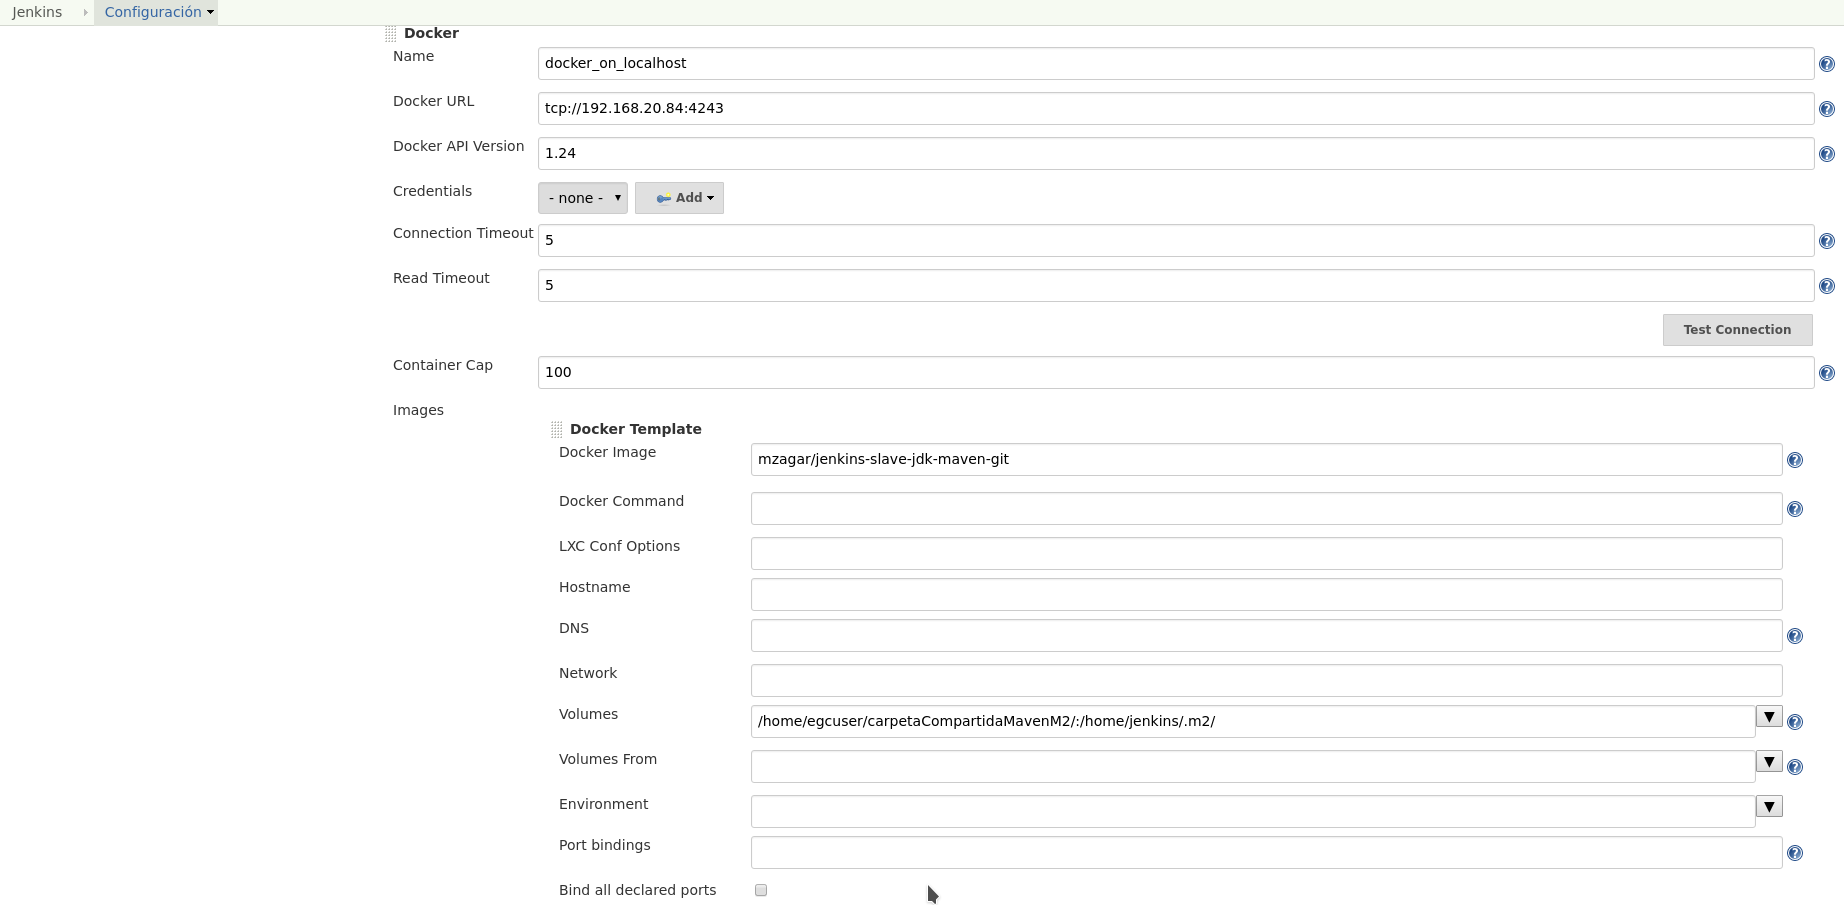
\includegraphics[width=4.7in]{images/jenkins/docker_slave_a/jenkins_dockerSlaveA_1.png}
	\end{center}
\end{frame}

\begin{frame}
	\frametitle{Fase Make - Jenkins Slave}
	\begin{center}
		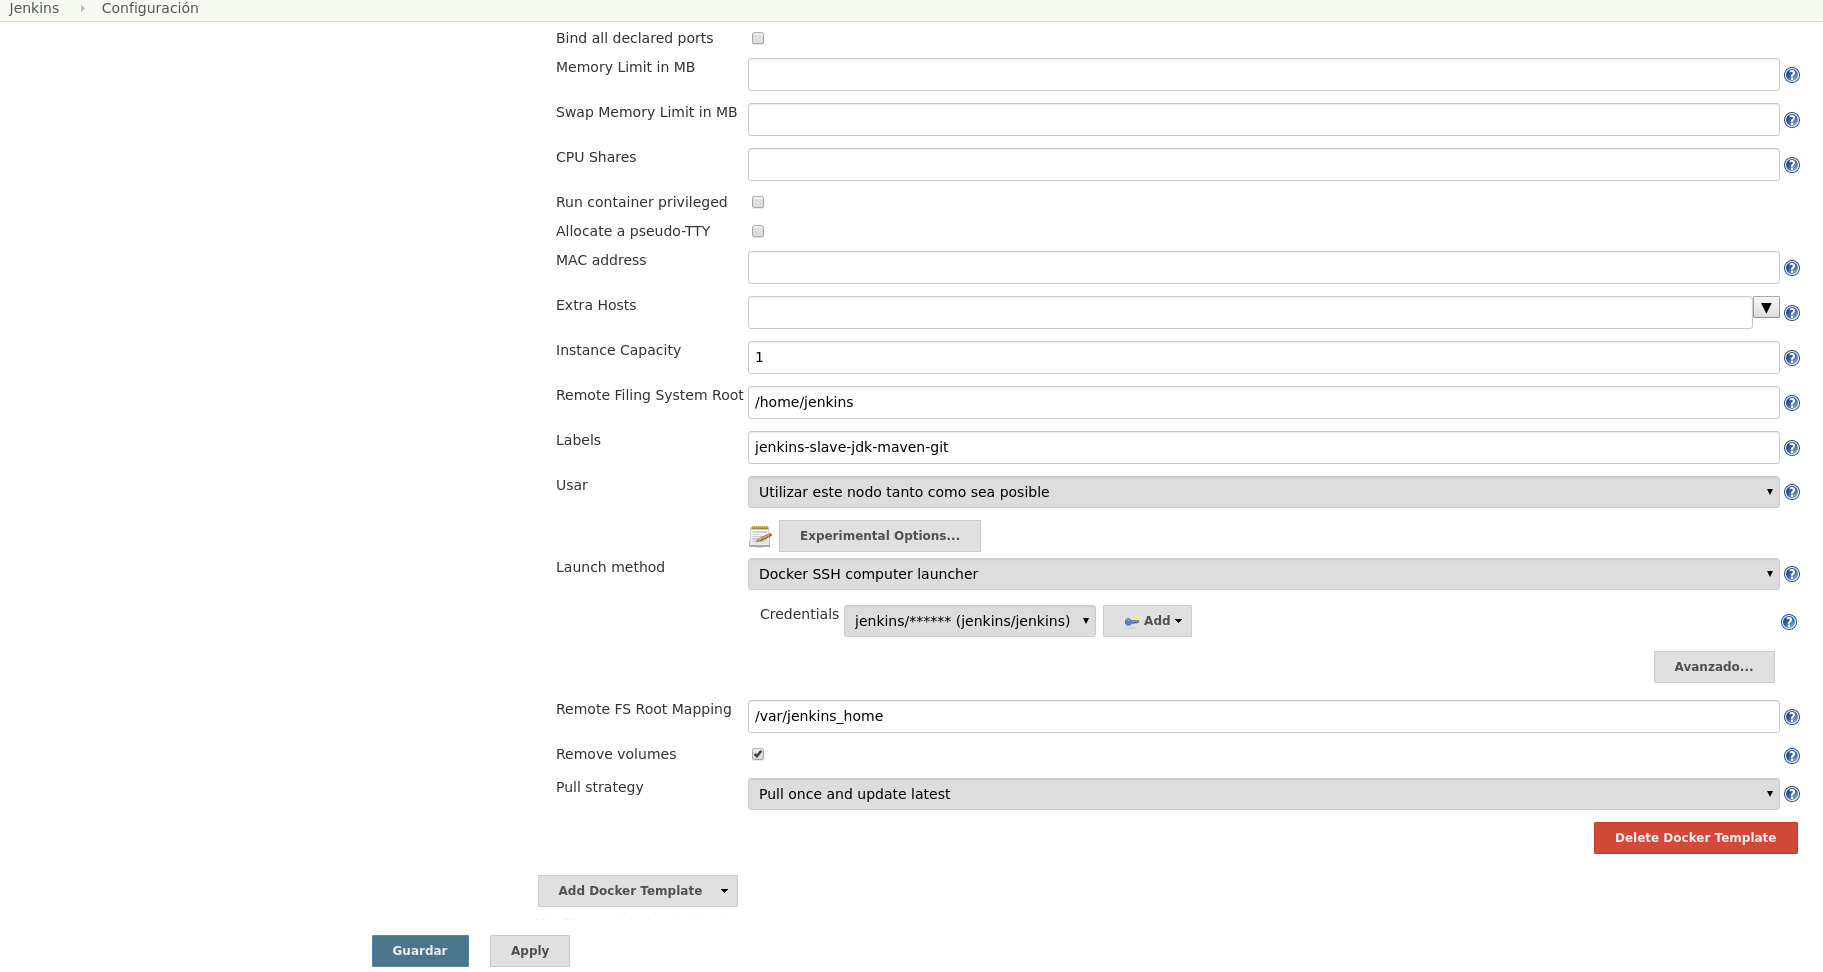
\includegraphics[width=4.7in]{images/jenkins/docker_slave_a/jenkins_dockerSlaveA_2.png}
	\end{center}
\end{frame}

\begin{frame}
	\frametitle{Fase Make - Jenkins Job Configure}
	\href{https://hub.docker.com/r/mzagar/jenkins-slave-jdk-maven-git/}{Imagen en DockerHub}
	
	\vspace{0.5in}
	\href{https://github.com/mzagar/jenkins-slave-jdk-maven-git}{Imagen en GitHub}
\end{frame}

\begin{frame}
	\frametitle{Fase Make - Jenkins Job Configure}
	\begin{center}
		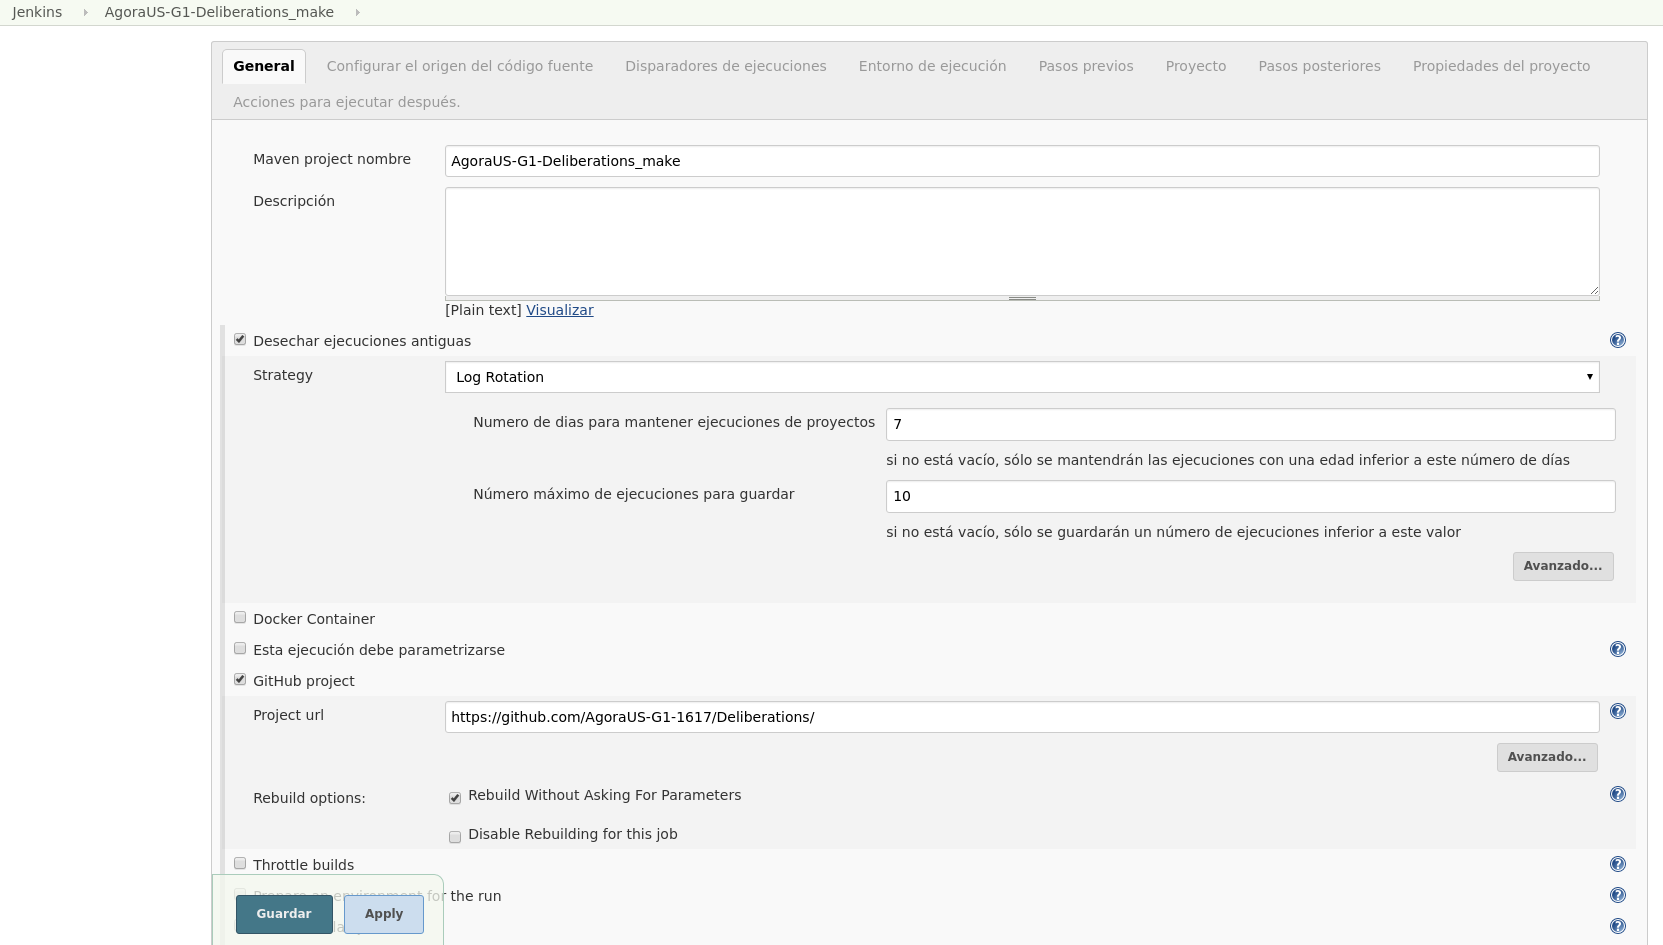
\includegraphics[width=4.7in]{images/jenkins/make_a/jenkins_makeA_1.png}
	\end{center}
\end{frame}

\begin{frame}
	\frametitle{Fase Make - Jenkins Job Configure}
	\begin{center}
		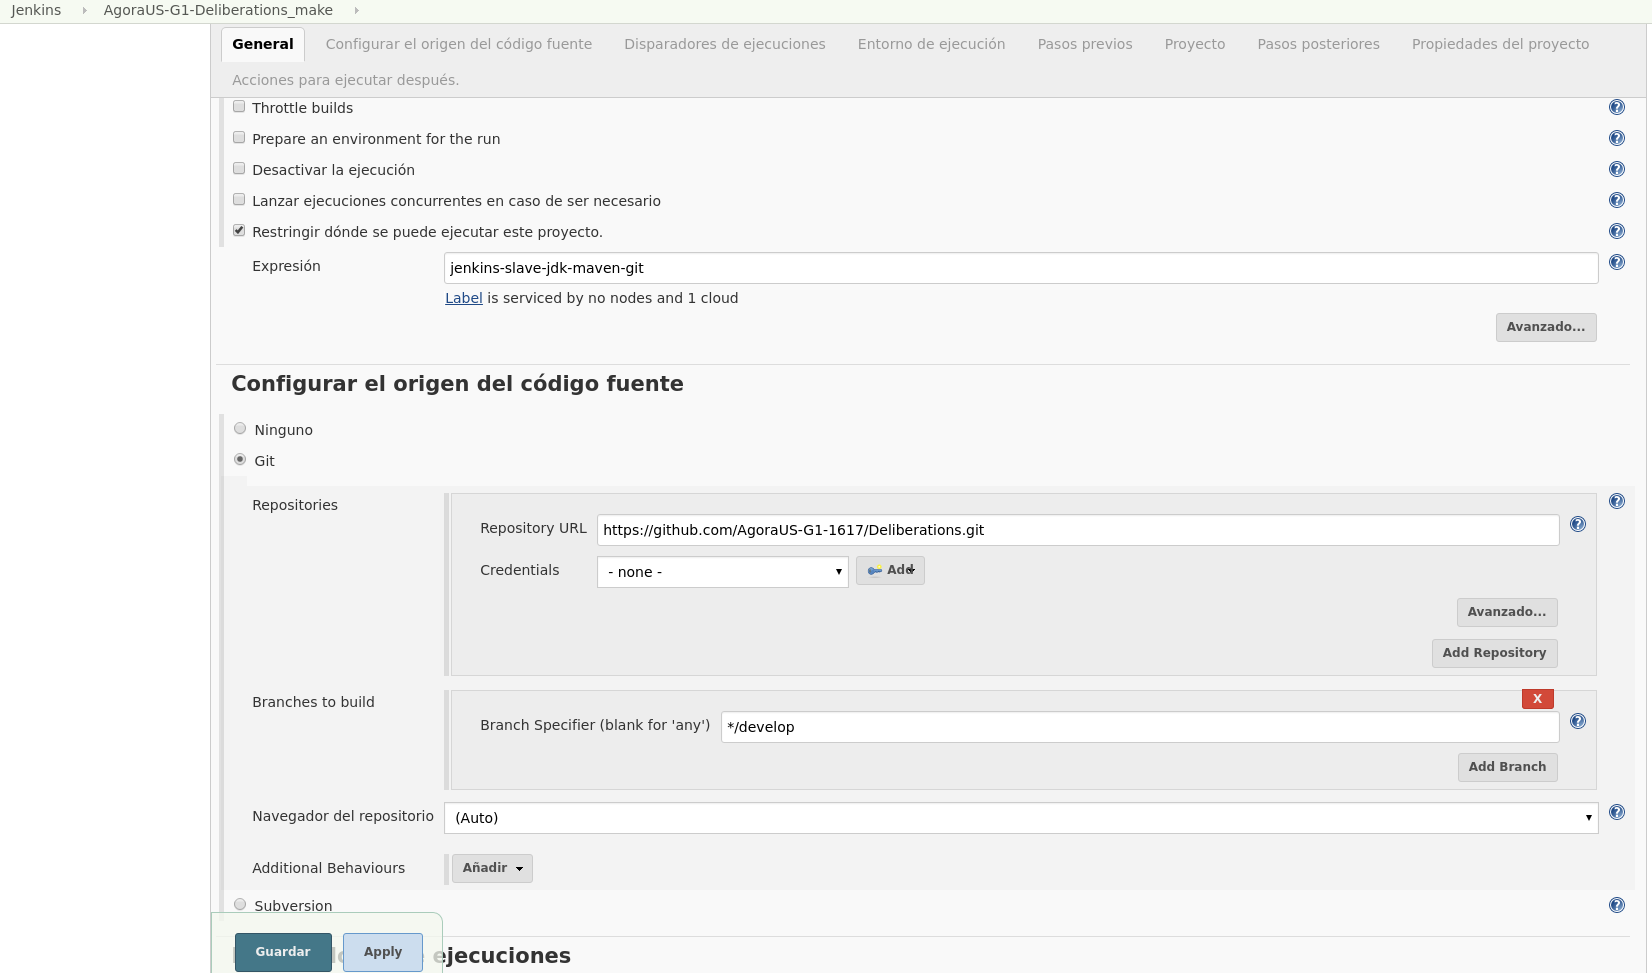
\includegraphics[width=4.7in]{images/jenkins/make_a/jenkins_makeA_2.png}
	\end{center}
\end{frame}

\begin{frame}
	\frametitle{Fase Make - Jenkins Job Configure}
	\begin{center}
		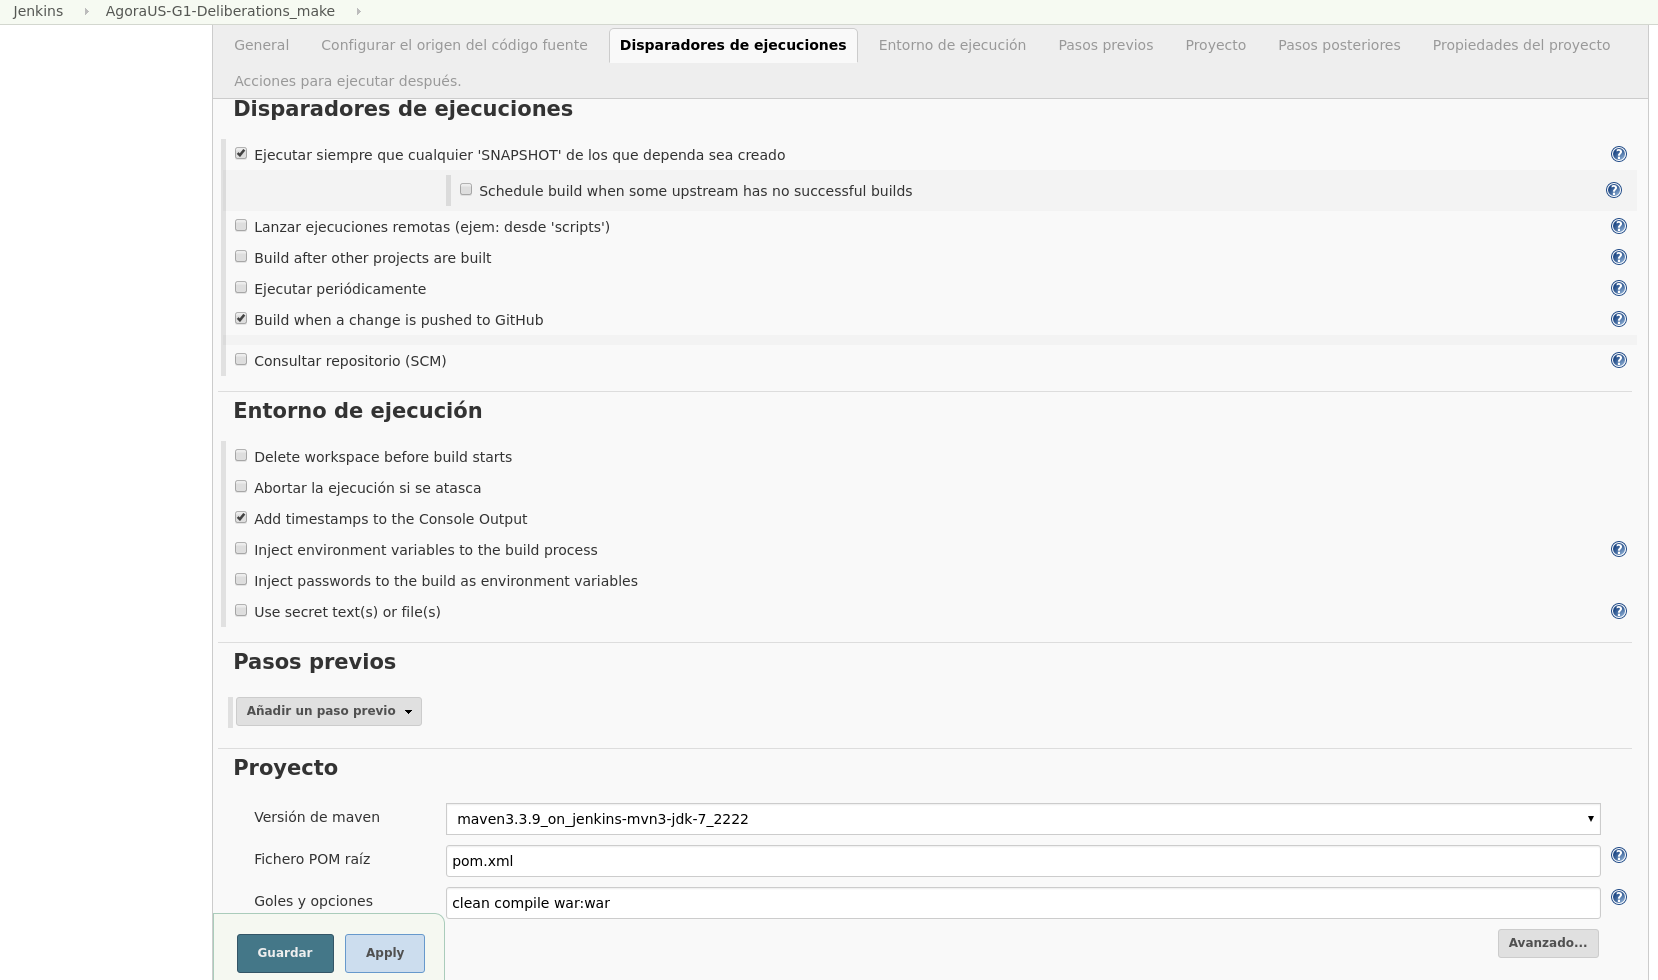
\includegraphics[width=4.7in]{images/jenkins/make_a/jenkins_makeA_3.png}
	\end{center}
\end{frame}

\begin{frame}
	\frametitle{Fase Make - Jenkins Job Configure}
	%Acabar remarcardando que se copiará el archivo de config en el repo para que quede constancia de como debe ser
	\begin{center}
		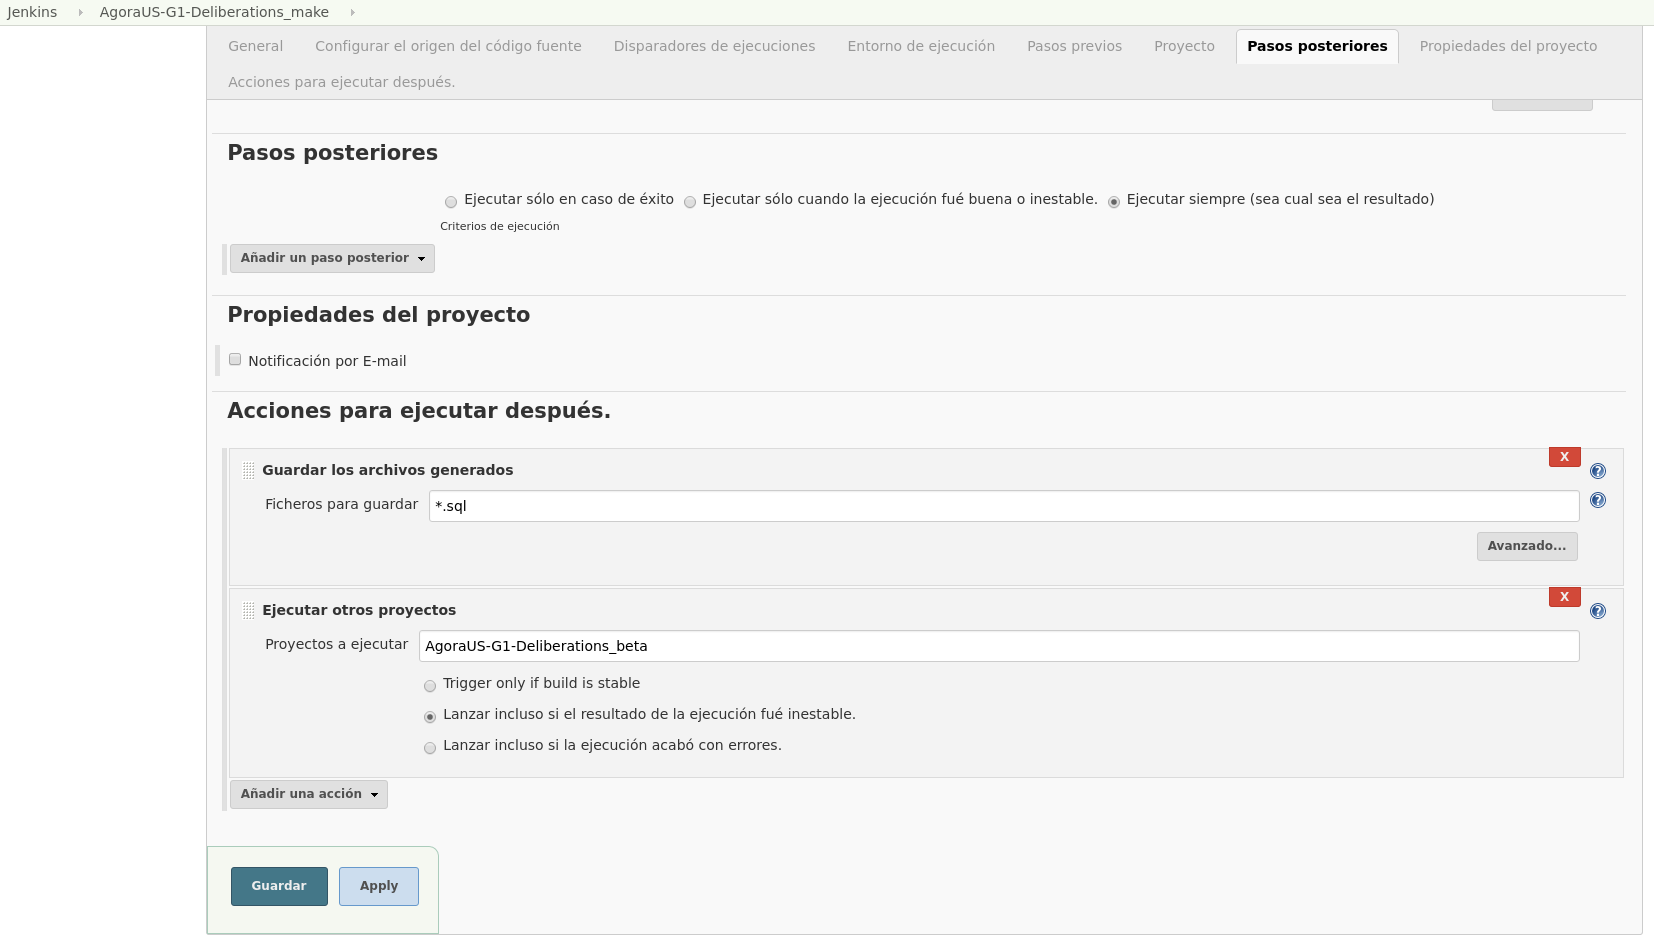
\includegraphics[width=4.7in]{images/jenkins/make_a/jenkins_makeA_4.png}
	\end{center}
\end{frame}

\begin{frame}
	\frametitle{Fase Make - Jenkins Job Configure}
	Es aconsejable copiar el archivo de configuración del trabajo generado por jenkins al repositorio con el fin de facilitar la restauración de la configuración.
	
	\vspace{0.2in}
%	Ruta: JENKINS\_HOME/jobs/\left[JOBNAME\right]/config.xml

%	Ruta: JENKINS_HOME/jobs/[JOBNAME]/config.xml
	% Concluir remarcardando que se copiará el archivo de config en el repo para que quede constancia de como debe ser

\end{frame}


\subsubsection{Fase Beta}
\begin{frame}
	\frametitle{Fase Beta - Jenkins Job Configure}
	\begin{center}
		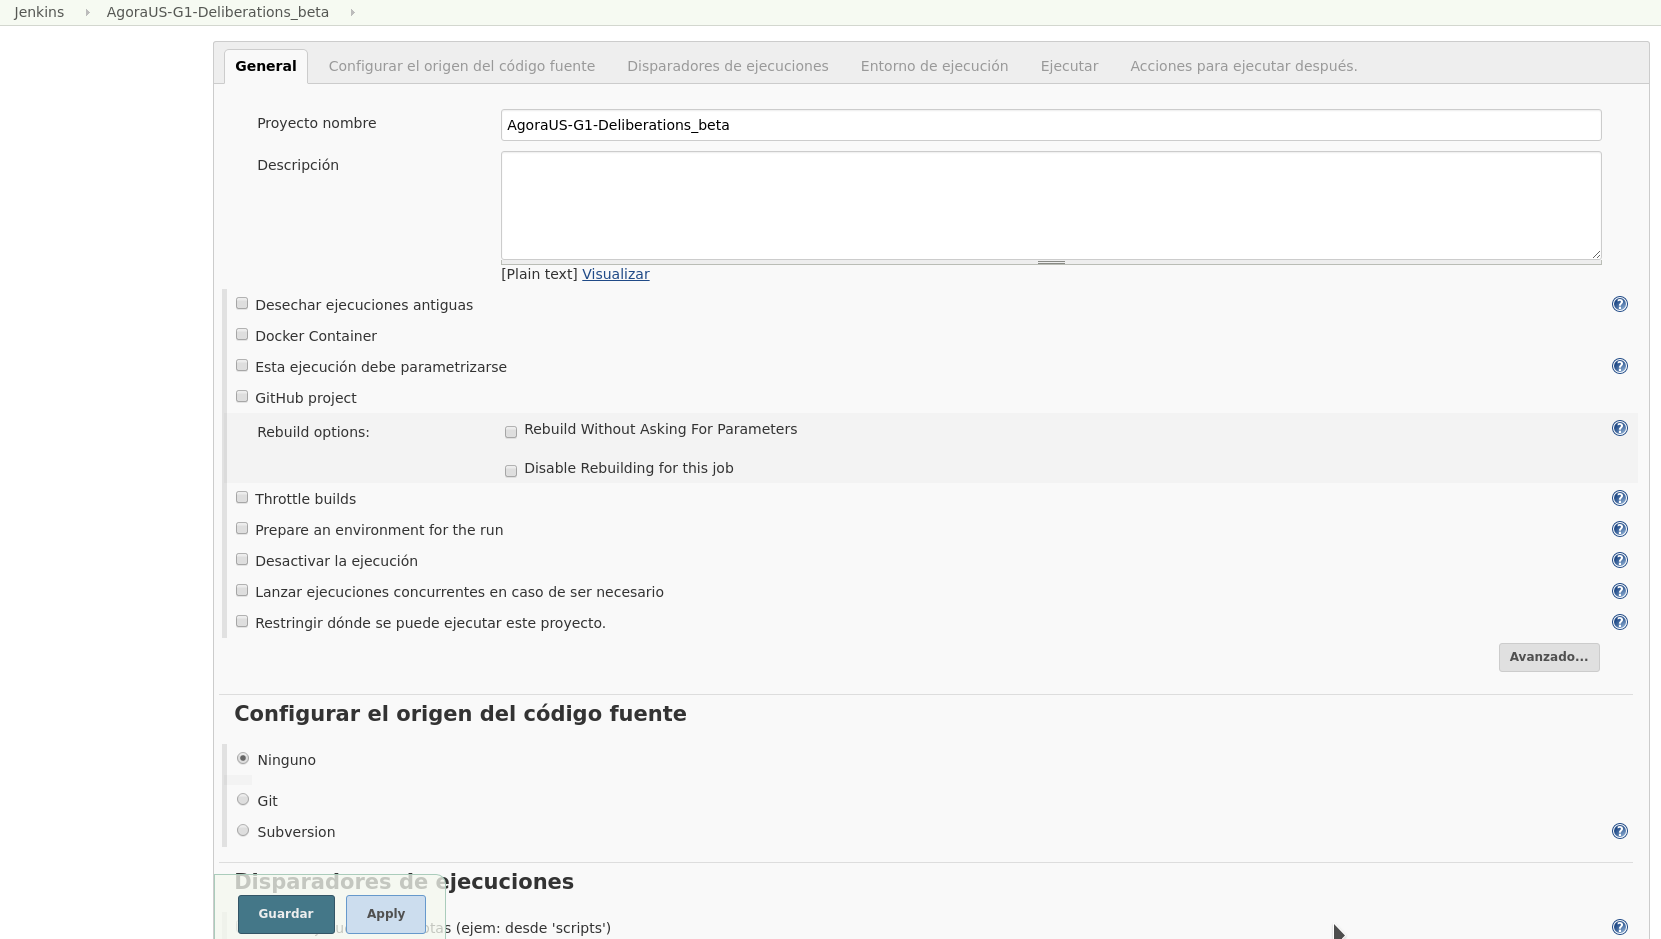
\includegraphics[width=4.7in]{images/jenkins/beta_a/jenkins_betaA_1.png}
	\end{center}
\end{frame}

\begin{frame}
	\frametitle{Fase Beta - Jenkins Job Configure}
	\begin{center}
		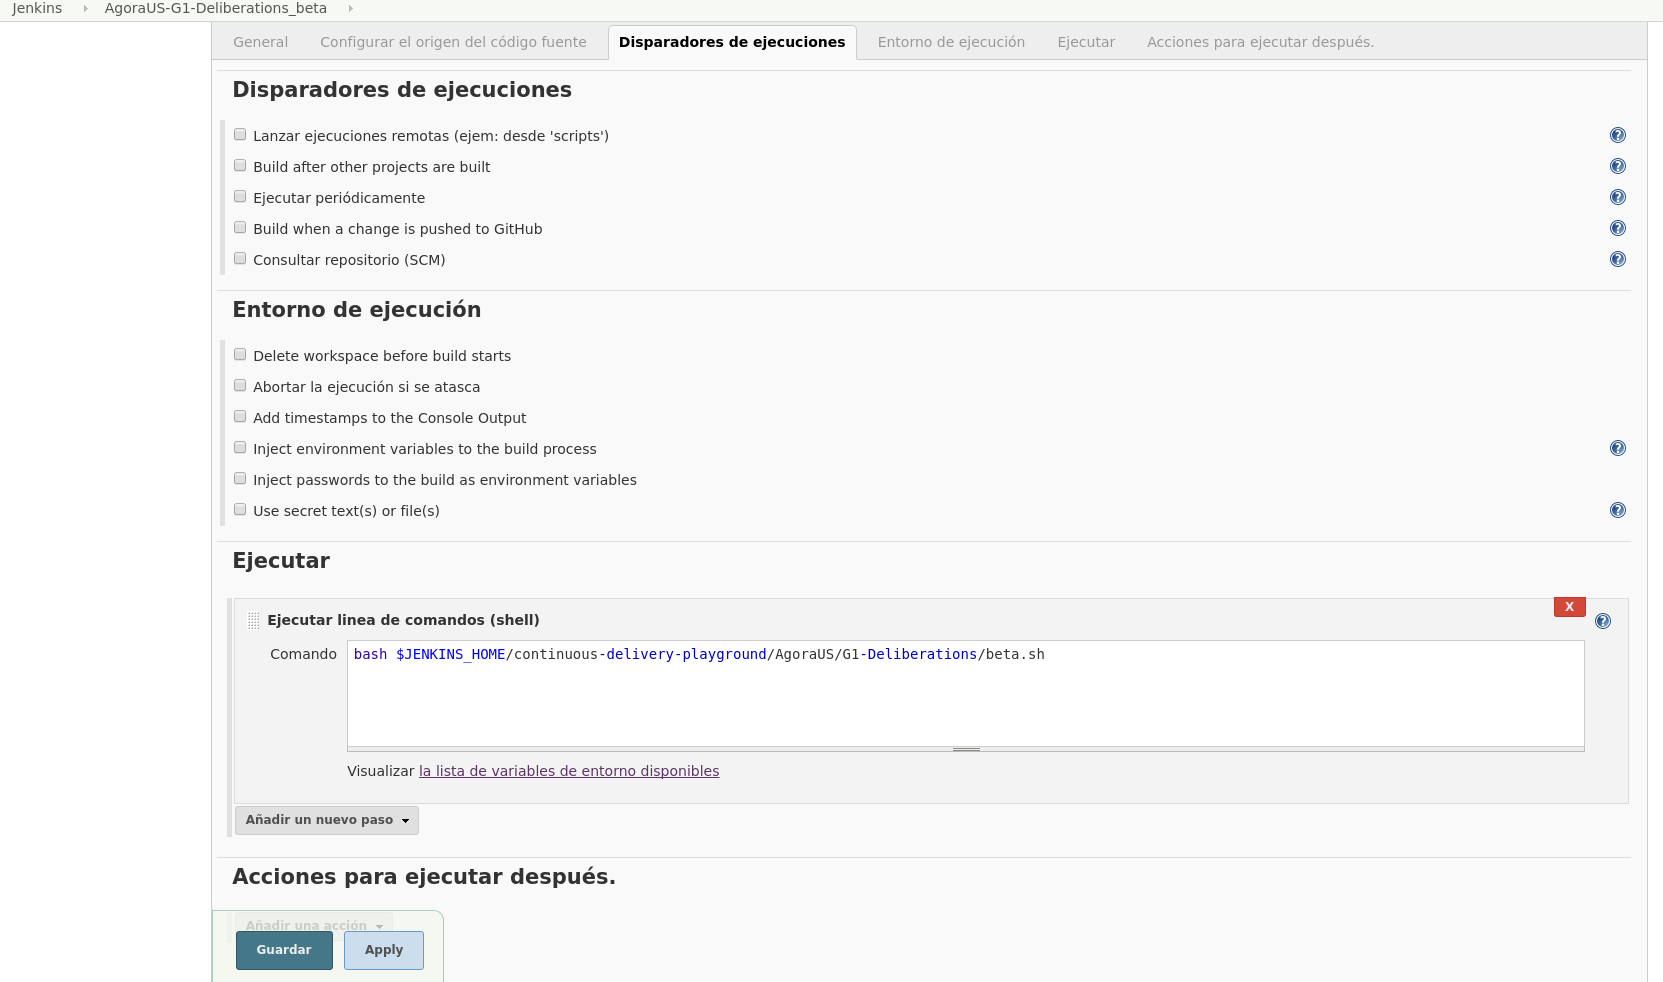
\includegraphics[width=4.7in]{images/jenkins/beta_a/jenkins_betaA_2.png}
	\end{center}
\end{frame}

\begin{frame}[fragile]
	\frametitle{Fase Beta - Jenkins Job Configure}
	%Fotos de config de jenkins 
	%Mostrar el código y las carpeta de la config

	\begin{itemize}
		\item \href{https://github.com/AgoraUS-G1-1617/continuous-integration-agoraus_g1/blob/master/AgoraUS/G1-Deliberations/beta.sh}{AgoraUS/G1-Deliberations/beta.sh}
		\item \href{https://hub.docker.com/_/mysql/}{Imagen MySQL}
		\item \href{https://hub.docker.com/_/tomcat/}{Imagen Tomcat}
	\end{itemize}
	
	
%	\begin{minted}{bash}
%		kate ../AgoraUS/G1-Deliberations/beta.sh
%	\end{minted}
	
\end{frame}


\begin{frame}[allowframebreaks]
	\frametitle{Referencias}

	\bibliographystyle{plain}
	\bibliography{presentation} 


\end{frame}


\end{document}
